\documentclass{standalone}

\usepackage{tikz}
\usetikzlibrary{arrows}

\begin{document}

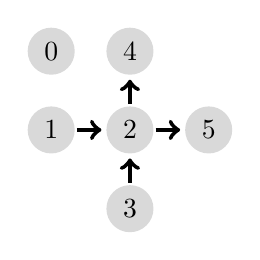
\begin{tikzpicture}[shorten >=1pt,->,ultra thick]
		\tikzstyle{vertex}=[circle,fill=black!15,minimum size=17pt,inner sep=0pt]
		\node[vertex] (0) at (0, 0) {$0$};    
		\node[vertex] (1) at (0,-1) {$1$};    
		\node[vertex] (4) at (1, 0) {$4$};      
		\node[vertex] (2) at (1,-1) {$2$};  
		\node[vertex] (5) at (2,-1) {$5$};  
		\node[vertex] (3) at (1,-2) {$3$};  

		\draw (1) -- (2);
		\draw (3) -- (2);
		\draw (2) -- (4); 
		\draw (2) -- (5);  
\end{tikzpicture}

\end{document}
